\PassOptionsToPackage{unicode=true}{hyperref} % options for packages loaded elsewhere
\PassOptionsToPackage{hyphens}{url}
\documentclass[11pt,dvipsnames,ignorenonframetext,aspectratio=169]{beamer}
\IfFileExists{pgfpages.sty}{\usepackage{pgfpages}}{}
\setbeamertemplate{caption}[numbered]
\setbeamertemplate{caption label separator}{: }
\setbeamercolor{caption name}{fg=normal text.fg}
\beamertemplatenavigationsymbolsempty
\usepackage{lmodern}
\usepackage{amssymb,amsmath}
\usepackage{ifxetex,ifluatex}
\usepackage{fixltx2e} % provides \textsubscript
\ifnum 0\ifxetex 1\fi\ifluatex 1\fi=0 % if pdftex
  \usepackage[T1]{fontenc}
  \usepackage[utf8]{inputenc}
\else % if luatex or xelatex
  \ifxetex
    \usepackage{mathspec}
  \else
    \usepackage{fontspec}
\fi
\defaultfontfeatures{Ligatures=TeX,Scale=MatchLowercase}







\fi

  \usetheme[]{monash}

  \usecolortheme{monashwhite}


% A default size of 24 is set in beamerthememonash.sty


  \useinnertheme{rounded}

  \useoutertheme{smoothtree}

% use upquote if available, for straight quotes in verbatim environments
\IfFileExists{upquote.sty}{\usepackage{upquote}}{}
% use microtype if available
\IfFileExists{microtype.sty}{%
  \usepackage{microtype}
  \UseMicrotypeSet[protrusion]{basicmath} % disable protrusion for tt fonts
}{}


\newif\ifbibliography


\hypersetup{
      pdftitle={Hybrid maize comprehensive technologies},
            colorlinks=true,
    linkcolor=red,
    citecolor=Blue,
    urlcolor=lightgrayd,
    breaklinks=true}
%\urlstyle{same}  % Use monospace font for urls







% Prevent slide breaks in the middle of a paragraph:
\widowpenalties 1 10000
\raggedbottom

  \AtBeginPart{
    \let\insertpartnumber\relax
    \let\partname\relax
    \frame{\partpage}
  }
  \AtBeginSection{
    \ifbibliography
    \else
      \let\insertsectionnumber\relax
      \let\sectionname\relax
      \frame{\sectionpage}
    \fi
  }
  \AtBeginSubsection{
    \let\insertsubsectionnumber\relax
    \let\subsectionname\relax
    \frame{\subsectionpage}
  }



\setlength{\parindent}{0pt}
\setlength{\parskip}{6pt plus 2pt minus 1pt}
\setlength{\emergencystretch}{3em}  % prevent overfull lines
\providecommand{\tightlist}{%
  \setlength{\itemsep}{0pt}\setlength{\parskip}{0pt}}

  \setcounter{secnumdepth}{0}


%% Monash overrides
\AtBeginSection[]{
   \frame<beamer>{
   \frametitle{Outline}\vspace*{0.2cm}
   
   \tableofcontents[currentsection,hideallsubsections]
  }}

% Redefine shaded environment if it exists (to ensure text is black)
\ifcsname Shaded\endcsname
  \definecolor{shadecolor}{RGB}{225,225,225}
  \renewenvironment{Shaded}{\color{black}\begin{snugshade}\color{black}}{\end{snugshade}}
\fi
%%

  \usepackage{setspace}
  \usepackage{wasysym}
  % \usepackage{footnote} % don't use this this breaks all
  \usepackage{fontenc}
  \usepackage{fontawesome}
  \usepackage{booktabs,siunitx}
  \usepackage{longtable}
  \usepackage{array}
  \usepackage{multirow}
  \usepackage{wrapfig}
  \usepackage{float}
  \usepackage{colortbl}
  \usepackage{pdflscape}
  \usepackage{tabu}
  \usepackage{threeparttable}
  \usepackage{threeparttablex}
  \usepackage[normalem]{ulem}
  \usepackage{makecell}
  \usepackage{xcolor}
  \usepackage{tikz} % required for image opacity change
  \usepackage[absolute,overlay]{textpos} % for text formatting
  \usepackage{chemfig}
  
  \floatplacement{figure}{H}
  
  % Added by CII
  \usepackage[format=hang,labelfont=bf,margin=0.5cm,justification=centering]{caption}
  \captionsetup{font=small,width=0.9\linewidth,labelfont=small,textfont={small,bf}}
  % End of CII addition
  
  \usepackage{subcaption}
  \newcommand{\subfloat}[2][need a sub-caption]{\subcaptionbox{#1}{#2}}
  
  % \captionsetup[sub]{font=footnotesize}
  \captionsetup[subfigure]{font=small,labelfont=small,textfont=small}
  
  % \newcommand*{\AlignChar}[1]{\makebox[1ex][c]{\ensuremath{\scriptstyle#1}}}%
  
  % this font option is amenable for beamer, although these are global settings
  \setbeamerfont{caption}{size=\tiny}
  \setbeamerfont{subcaption}{size=\tiny} % this is doubted if has any effects
  
  \singlespacing
  \definecolor{lightgrayd}{gray}{0.95}
  \definecolor{skyblued}{rgb}{0.65, 0.6, 0.94}
  \definecolor{oranged}{RGB}{245, 145, 200}
  
  % define new column types (say, L, C, and R) that take their width as argument and do the following
  % - Issue \raggedright, \centering, or \raggedleft to achieve the desired horizontal alignment,
  % - Declare \let\newline\\ to allow to use \newline for manual line breaks within a cell (note that \centering & friends change the meaning of \\ -- this is the problem with Jake's solution),
  % - Issue \arraybackslash (i.e., \let\\\tabularnewline) to allow (again) to use \\ for ending rows,
  % - Issue \hspace{0pt} to allow the first word in a cell to be hyphenated.
  \newcolumntype{R}[1]{>{\raggedleft\let\newline\\\arraybackslash\hspace{0pt}}p{#1}}
  \newcolumntype{L}[1]{>{\raggedright\let\newline\\\arraybackslash\hspace{0pt}}m{#1}}
  \newcolumntype{C}[1]{>{\centering\let\newline\\\arraybackslash\hspace{0pt}}m{#1}}
  
  % Added by CII
  %%% Copied from knitr
  %% maxwidth is the original width if it's less than linewidth
  %% otherwise use linewidth (to make sure the graphics do not exceed the margin)
  \makeatletter
  \def\maxwidth{ %
    \ifdim\Gin@nat@width>\linewidth
      \linewidth
    \else
      \Gin@nat@width
    \fi
  }
  \makeatother
  
  \usepackage{background}

  \title[]{Hybrid maize comprehensive technologies}


  \author[
        \textit{ddhakal.rookie@gmail.com}\\
\url{https://rookie.rbind.io}
    ]{\textit{ddhakal.rookie@gmail.com}\\
\url{https://rookie.rbind.io}}


\date[
      Academic year 2019-2020
  ]{
      Academic year 2019-2020
        }

\begin{document}

% Hide progress bar and footline on titlepage
  \begin{frame}[plain]
  \titlepage
  \end{frame}


   \frame<beamer>{
   \frametitle{Outline}\vspace*{0.2cm}
   
   \tableofcontents[hideallsubsections]
  }

\hypertarget{maize-genetics-and-breeding}{%
\section{Maize genetics and
breeding}\label{maize-genetics-and-breeding}}

\begin{frame}{Basic situation of maize breeding}
\protect\hypertarget{basic-situation-of-maize-breeding}{}

\begin{itemize}
\tightlist
\item
  Only 7 hybrids released so far in Nepal
\item
  National Seed Vision envisions national production scenario
  strengthened through hybrid development (9+5)
\end{itemize}

\end{frame}

\begin{frame}{Main problems of maize breeding}
\protect\hypertarget{main-problems-of-maize-breeding}{}

\begin{itemize}
\tightlist
\item
  White colored national hybrids lacking
\item
  Proper database of inbred lines their characterization lacking
\item
  Research in heterotic pattern un-sytematized regarding hybrid variety
  development
\item
  Competitive hybrid maize seed production technology lacking
\end{itemize}

\end{frame}

\begin{frame}{General objectives of maize breeding}
\protect\hypertarget{general-objectives-of-maize-breeding}{}

\begin{itemize}
\tightlist
\item
  High yield and good quality
\item
  Stable yield
\item
  Proper growth duration
\item
  Easing mechanization
\item
  Various Stresses tolerant varieties development
\end{itemize}

\end{frame}

\begin{frame}{Inheritance of traits in Maize}
\protect\hypertarget{inheritance-of-traits-in-maize}{}

\begin{itemize}
\tightlist
\item
  Qualitative traits:

  \begin{itemize}
  \tightlist
  \item
    grain type and color, endosperm quality, silk color, ligule, and
    resistance to some diseases
  \end{itemize}
\item
  Quantitative traits:

  \begin{itemize}
  \tightlist
  \item
    yield, growth duration, and ear length, 1000-grains-weight, plant
    type
  \end{itemize}
\end{itemize}

\end{frame}

\begin{frame}{Hybridization techniques in Maize}
\protect\hypertarget{hybridization-techniques-in-maize}{}

\begin{itemize}
\tightlist
\item
  Materials
\item
  Procedures in pollination
\item
  Techniques of hybridization
\item
  Use of MS lines
\item
  Manual pollination
\end{itemize}

\end{frame}

\begin{frame}{Future Direction of Maize Breeding Program}
\protect\hypertarget{future-direction-of-maize-breeding-program}{}

\begin{itemize}
\tightlist
\item
  Heterotic group patterning
\item
  Acquisition of high yielding Inbred lines.
\item
  Fostering collaboration of National Research Program and seed
  production as well as commercial sectors (Public and Private sectors)
\end{itemize}

\end{frame}

\hypertarget{maize-cultivation-technology}{%
\section{Maize cultivation
technology}\label{maize-cultivation-technology}}

\begin{frame}{Open field and direct seedling cultivation}
\protect\hypertarget{open-field-and-direct-seedling-cultivation}{}

\begin{itemize}
\tightlist
\item
  Seedling period: Spring, Summer and Autumn
\item
  Seedling at proper time, reasonable close planting, planting methods
  (equal width between lines, single plant in one cavity, equal width
  between lines, double plants in each cavity, wide-narrow lines with
  single plant, strip intercropping), seeding quantity and depth,
  seeding quantity and depth
\item
  Field Management: Thinning, filling the gaps with seedlings and final
  singling, intertill, weeding and to earth up, fertilization
  (Stem-oriented fertilization, Ear-oriented fertilization,
  Grain-oriented fertilization), irrigation and drainage, removing
  tillerings, artificial supplementary pollination, prevention and
  treatment of diseases and insect pests, harvesting and storage,
\end{itemize}

\end{frame}

\begin{frame}{Precocious high-yield maize with plastic film mulching}
\protect\hypertarget{precocious-high-yield-maize-with-plastic-film-mulching}{}

\begin{itemize}
\tightlist
\item
  The cultivation technology of precocious high-yield maize with plastic
  film mulching.
\item
  Selecting maize variety suitable for plastic film mulching
\item
  Early planting within proper range
\item
  Mulching
\item
  Free the seedlings
\item
  Field management
\end{itemize}

\end{frame}

\hypertarget{machinery-in-china}{%
\section{Machinery in China}\label{machinery-in-china}}

\begin{frame}{}
\protect\hypertarget{section}{}

\begin{figure}[H]
\subfloat[Stubble cleaner\label{fig:corn-field-management-machinery1}]{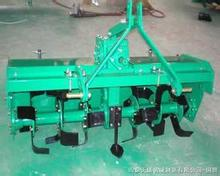
\includegraphics[width=.25\linewidth]{./images/stubble_cleaner} }\subfloat[Small scale maize sower\label{fig:corn-field-management-machinery2}]{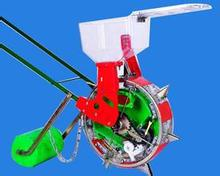
\includegraphics[width=.25\linewidth]{./images/small_scale_maize_sower} }\subfloat[Maize sower operating on field\label{fig:corn-field-management-machinery3}]{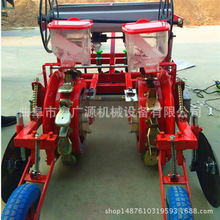
\includegraphics[width=.25\linewidth]{./images/maize_sower} }\subfloat[Mulch applicator\label{fig:corn-field-management-machinery4}]{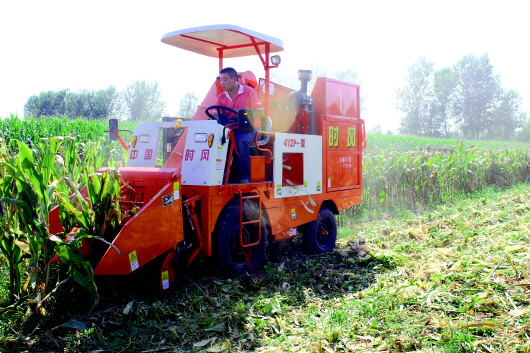
\includegraphics[width=.25\linewidth]{./images/mulch_applicator} }\caption{Gallery of images showing machineries and implements for crop and harvest management of Corn}\label{fig:corn-field-management-machinery}
\end{figure}

\end{frame}

\begin{frame}{}
\protect\hypertarget{section-1}{}

\begin{figure}[H]
\subfloat[Maize drier bin\label{fig:corn-field-management-machinery21}]{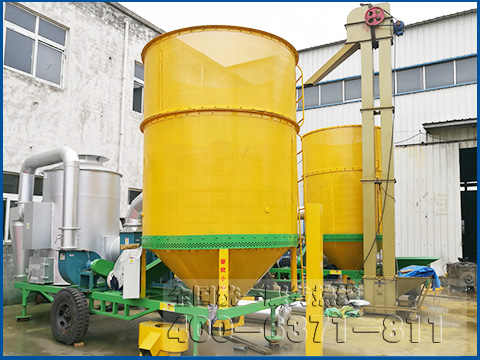
\includegraphics[width=.25\linewidth]{./images/maize_drier_bin} }\subfloat[Small scale maize kernel drier\label{fig:corn-field-management-machinery22}]{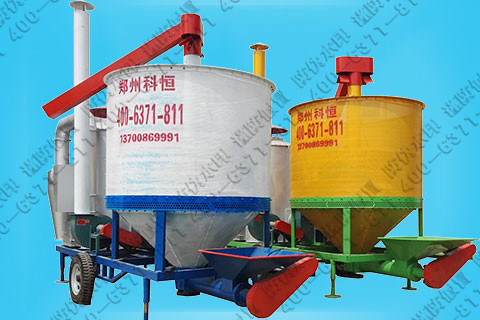
\includegraphics[width=.25\linewidth]{./images/small_scale_drier} }\subfloat[Direct maize sower\label{fig:corn-field-management-machinery23}]{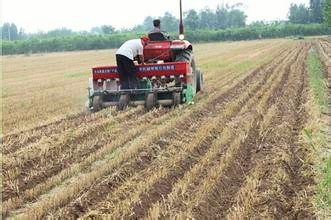
\includegraphics[width=.25\linewidth]{./images/direct_maize_sower} }\caption{Gallery of images showing machineries and implements for crop and harvest management of Corn}\label{fig:corn-field-management-machinery2}
\end{figure}

\end{frame}

\hypertarget{corn-processing}{%
\section{Corn processing}\label{corn-processing}}

\begin{frame}{Upstream products}
\protect\hypertarget{upstream-products}{}

\begin{itemize}
\tightlist
\item
  Corn Kernel

  \begin{itemize}
  \tightlist
  \item
    Corn starch
  \item
    Corn gluten
  \item
    Corn germ cake
  \item
    Corn fiber
  \item
    Corn steep liquor
  \end{itemize}
\end{itemize}

\end{frame}

\begin{frame}{Downstream products}
\protect\hypertarget{downstream-products}{}

\begin{itemize}
\tightlist
\item
  Corn Kernel

  \begin{itemize}
  \tightlist
  \item
    Corn Starch
  \item
    Amino Acids
  \item
    Corn Sweeteners
  \item
    Modified Starches
  \item
    Chemicals
  \end{itemize}
\end{itemize}

\end{frame}

\begin{frame}{Machinery}
\protect\hypertarget{machinery}{}

\begin{figure}[H]
\subfloat[Heap of corn\label{fig:corn-processing-machinery1}]{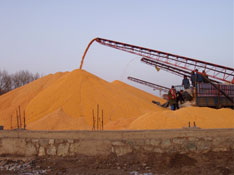
\includegraphics[width=.25\linewidth]{./images/mountain_of_corn} }\subfloat[Fiber separator\label{fig:corn-processing-machinery2}]{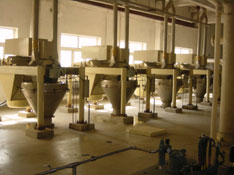
\includegraphics[width=.25\linewidth]{./images/fiber_separator} }\subfloat[Starch slurry extractor\label{fig:corn-processing-machinery3}]{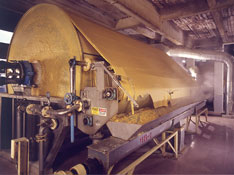
\includegraphics[width=.25\linewidth]{./images/starch_slurry_extraction} }\caption{Machinery and equipments for corn processing}\label{fig:corn-processing-machinery}
\end{figure}

\end{frame}

\begin{frame}{}
\protect\hypertarget{section-2}{}

\begin{figure}[H]
\subfloat[Machine for second grinding\label{fig:corn-processing-machinery21}]{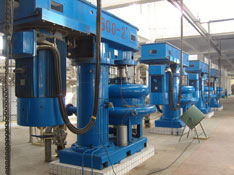
\includegraphics[width=.25\linewidth]{./images/machine_for_second_grinding} }\subfloat[Protein separation machine\label{fig:corn-processing-machinery22}]{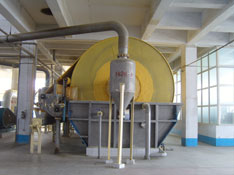
\includegraphics[width=.25\linewidth]{./images/protein_separation_machine} }\subfloat[Corn cleaning and dehydration facility\label{fig:corn-processing-machinery23}]{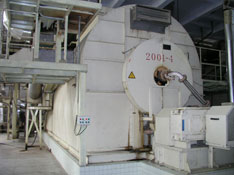
\includegraphics[width=.25\linewidth]{./images/corn_cleaning_dehydration_facility} }\caption{Machinery and equipments for corn processing}\label{fig:corn-processing-machinery2}
\end{figure}

\end{frame}

\hypertarget{environmental-factors-affecting-maize}{%
\section{Environmental factors affecting
maize}\label{environmental-factors-affecting-maize}}

\begin{frame}{}
\protect\hypertarget{section-3}{}

\begin{itemize}
\tightlist
\item
  Climatic and geographical factors

  \begin{itemize}
  \tightlist
  \item
    Water
  \item
    Geology
  \item
    Temperature: Maximum, Minimum
  \item
    Solar radiation: Solar intensity, Sunshine hours
  \end{itemize}
\item
  Soil factors

  \begin{itemize}
  \tightlist
  \item
    Nutrient content
  \item
    Soil profile
  \end{itemize}
\item
  Biotic factors

  \begin{itemize}
  \tightlist
  \item
    Diseases
  \item
    Pests
  \item
    Weeds
  \end{itemize}
\end{itemize}

\end{frame}

\begin{frame}{Ecological factors}
\protect\hypertarget{ecological-factors}{}

\begin{itemize}
\tightlist
\item
  Topography and geomorphology

  \begin{itemize}
  \tightlist
  \item
    shall be good for isolation, water irrigation \& drainage, and with
    enough sunlight exposure, conducive to prevention of wind and frost,
    and to soil fixation.
  \end{itemize}
\item
  Soil texture

  \begin{itemize}
  \tightlist
  \item
    Soil Type: sand, loam, clay-loam and clay, crumb structure,
    permeability\\
  \item
    Nutrient Structure
  \item
    Form of Nitrogen: the content and the existence of Protein, amino
    acids, humus, amide, or inorganic nitrogen like \(NO_3\) - and
    \(NO_2\) - and \(NH_4^+\) microbs, etc.
  \end{itemize}
\item
  Areas (1) with the occurence of serious pests (diseases and insects)
  or (2) with the high frequency of pests (diseases and insects)
  occurence or (3) with the occurency of pests (diseases and insects)
  which are regarded as quarantine objects shall not be used as the
  bases for seed production.
\end{itemize}

\end{frame}

\begin{frame}{Production level and seed growers' skills}
\protect\hypertarget{production-level-and-seed-growers-skills}{}

\begin{itemize}
\tightlist
\item
  Parental seed production base should be located in the areas with
  quite good agricultural production conditions and relatively high
  production level or the areas with crop production as the backbone of
  their economy.
\item
  Seed growers should have sound educational background, shall quickly
  accept new technologies of agricultural production, be ardent in
  absorbing new science and technologies and related seed know, be
  active in probing the agronomic technologies related to seed
  production, love the seed industry.
\end{itemize}

\end{frame}

\begin{frame}{Disease}
\protect\hypertarget{disease}{}

\begin{itemize}
\tightlist
\item
  Turcicum Leaf Blight,
\item
  Southern Leaf Blight,
\item
  Banded Leaf and Sheath Blight (BLSB)
\item
  Downy Mildew
\item
  Stalk rot
\item
  Penicilium ear rot
\item
  Diplodia Ear rot
\item
  Gray Speck disease
\item
  Rust disease
\item
  Scab in ear
\item
  Dwarf mosaic
\item
  Head smut
\end{itemize}

\end{frame}

\begin{frame}{Insect pests}
\protect\hypertarget{insect-pests}{}

\begin{itemize}
\tightlist
\item
  Thrips
\item
  White Grub
\item
  Armyworm
\item
  Corn Earworm
\item
  Pollen Beetle
\item
  Cutworm
\item
  Mole cricket
\item
  European corn borer
\item
  Aphids
\end{itemize}

\end{frame}

\hypertarget{seed-certification}{%
\section{Seed certification}\label{seed-certification}}

\begin{frame}{Criteria}
\protect\hypertarget{criteria}{}

\begin{itemize}
\tightlist
\item
  DUS test

  \begin{itemize}
  \tightlist
  \item
    with the distinguished characteristics of the typical traits are
    true of (consistent with) the typical traits of the parents of the
    breeder seeds, with uniform growth, high purity and high stability.
  \end{itemize}
\item
  Economic characters of the original level
\item
  Characters good enough for seeding:

  \begin{itemize}
  \tightlist
  \item
    complete maturity,\\
  \item
    high germination rate,
  \item
    no disease,
  \item
    no mildew,
  \item
    no pests of quarantine objects
  \end{itemize}
\end{itemize}

\end{frame}

\begin{frame}{Seed multiplication procedures are established according
to the degree of mixture (hybridization)}
\protect\hypertarget{seed-multiplication-procedures-are-established-according-to-the-degree-of-mixture-hybridization}{}

\begin{itemize}
\tightlist
\item
  The ``two-nursery system'' and the inbred line mixed multiplication
  with strict isolation are adopted in the production of parental seeds.
\item
  Direct multiplication from breeder seeds
\item
  Two-nursery system (when mixture degree is low)

  \begin{itemize}
  \tightlist
  \item
    selection of individual plant \& selfing,
  \item
    ear to row comparison,
  \item
    selection,
  \item
    bulk harvest
  \end{itemize}
\end{itemize}

\end{frame}

\hypertarget{note}{%
\section{Note}\label{note}}

\begin{frame}{Field visits and excursions}
\protect\hypertarget{field-visits-and-excursions}{}

\backgroundsetup{contents=Confidential,color=blue}

\begin{itemize}
\tightlist
\item
  NMRP: Crossing Block, Inbred Line Multiplication Plot
\item
  Seed Processing Unit of Lumbini Seed Company, Bhairahawa
\item
  Maize Superzone, Dang: Hybrid Maize Production Plot
\item
  Seed Producing Farmer's Group, Syangja: Seed Production of OPVs
  (Manakamana 3)
\item
  Ministry of Agriculture, Province 4
\item
  Lumle Regional Agriculture Research Station
\item
  Maize Demonstration Plot at Godawari: Waxy corn
\item
  NARC, Khumaltar: Agri-Botany Division (Field Visit of various Hybrid
  Maize Trials of ABD)
\end{itemize}

\end{frame}

\begin{frame}{}
\protect\hypertarget{section-4}{}

\begin{itemize}
\tightlist
\item
  This presentation is a group work, prepared by the ``Rhino'' group
  with following group members: Pratikshya Sharma, Bishnu Gautam,
  Damodar Gautam, Deepika Timsina, Sundar Shrestha, Deependra Dhakal,
  Abishek Shrestha, Anish Dahal, Ramesh Acharya, Maiya Giri, Debu
  Bhandari
\end{itemize}

\end{frame}

\begin{frame}{}
\protect\hypertarget{section-5}{}

\begin{figure}[H]
\subfloat[With RARS, Lumle team\label{fig:team-field-trips1}]{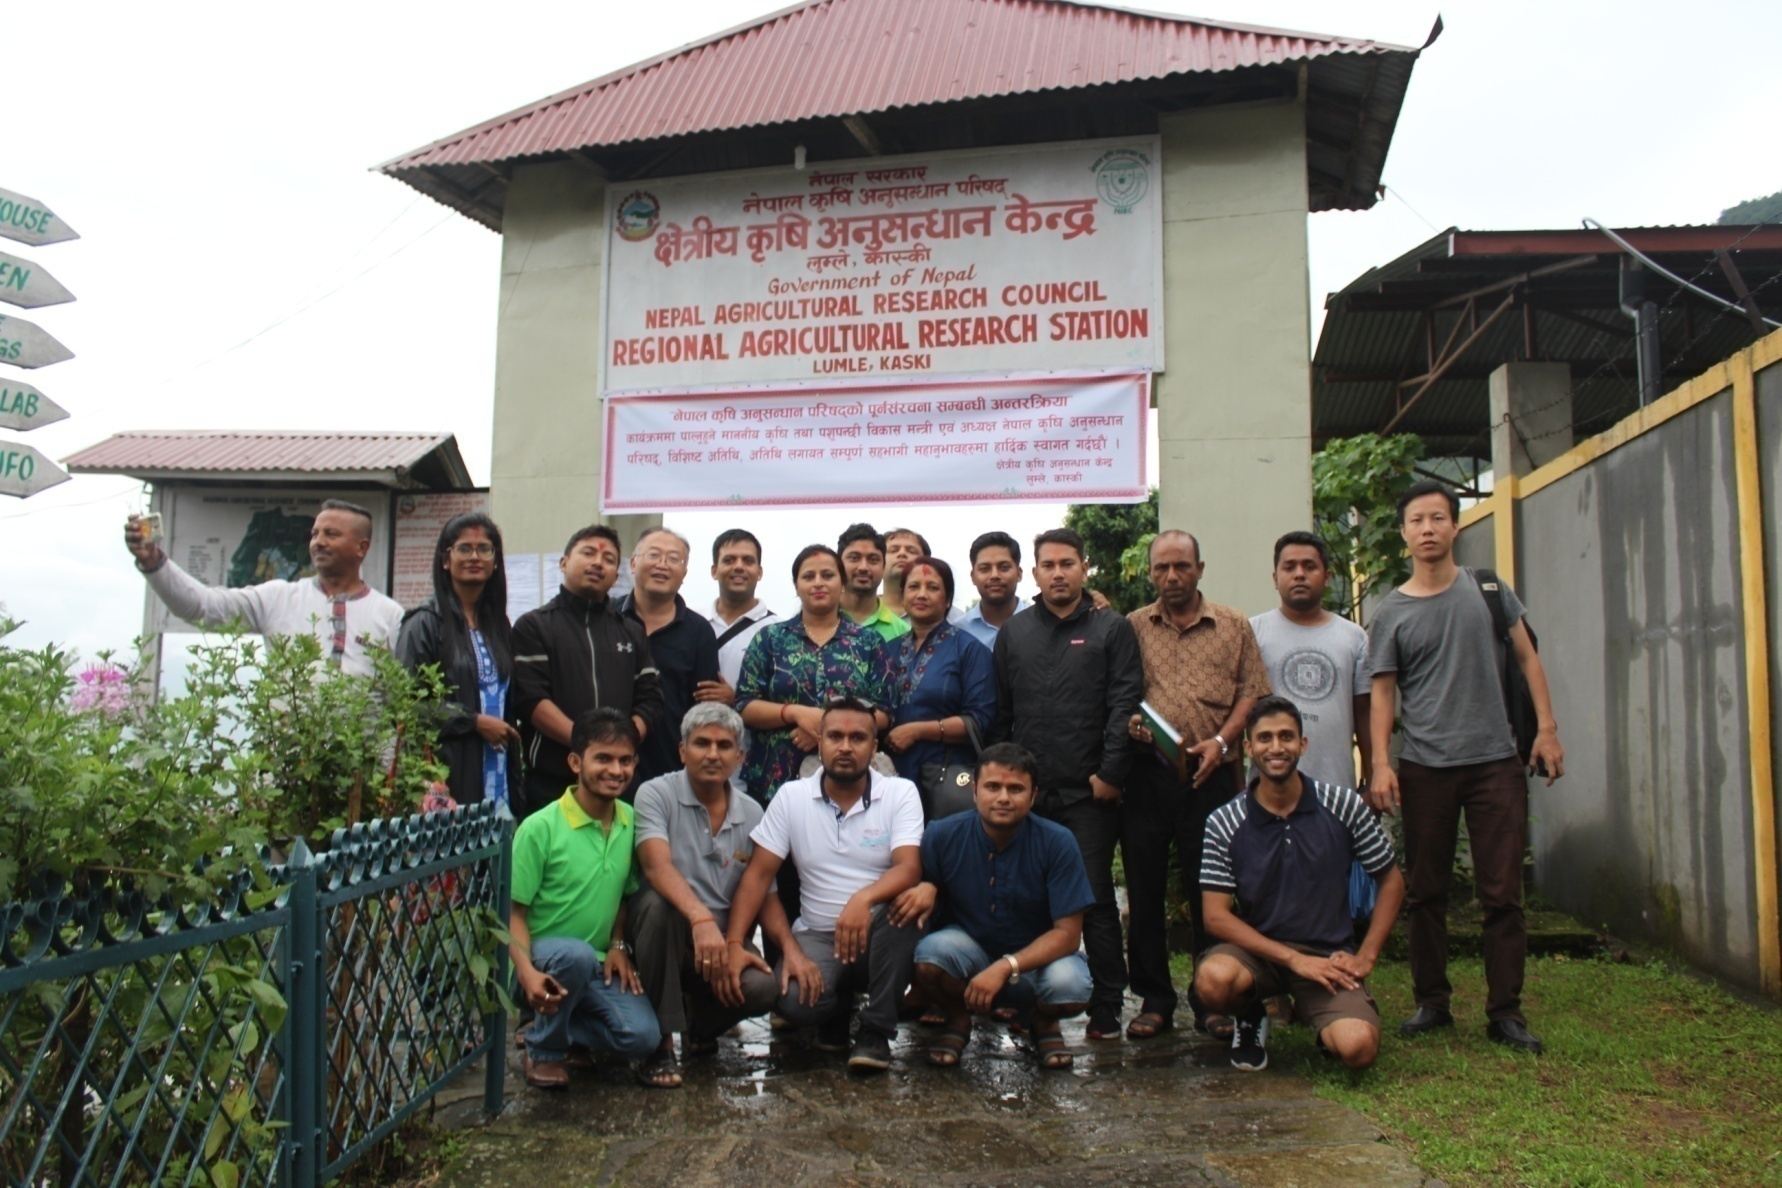
\includegraphics[width=.25\linewidth]{./images/rars_lumle_team} }\subfloat[Maize experiment field with disease screening trial\label{fig:team-field-trips2}]{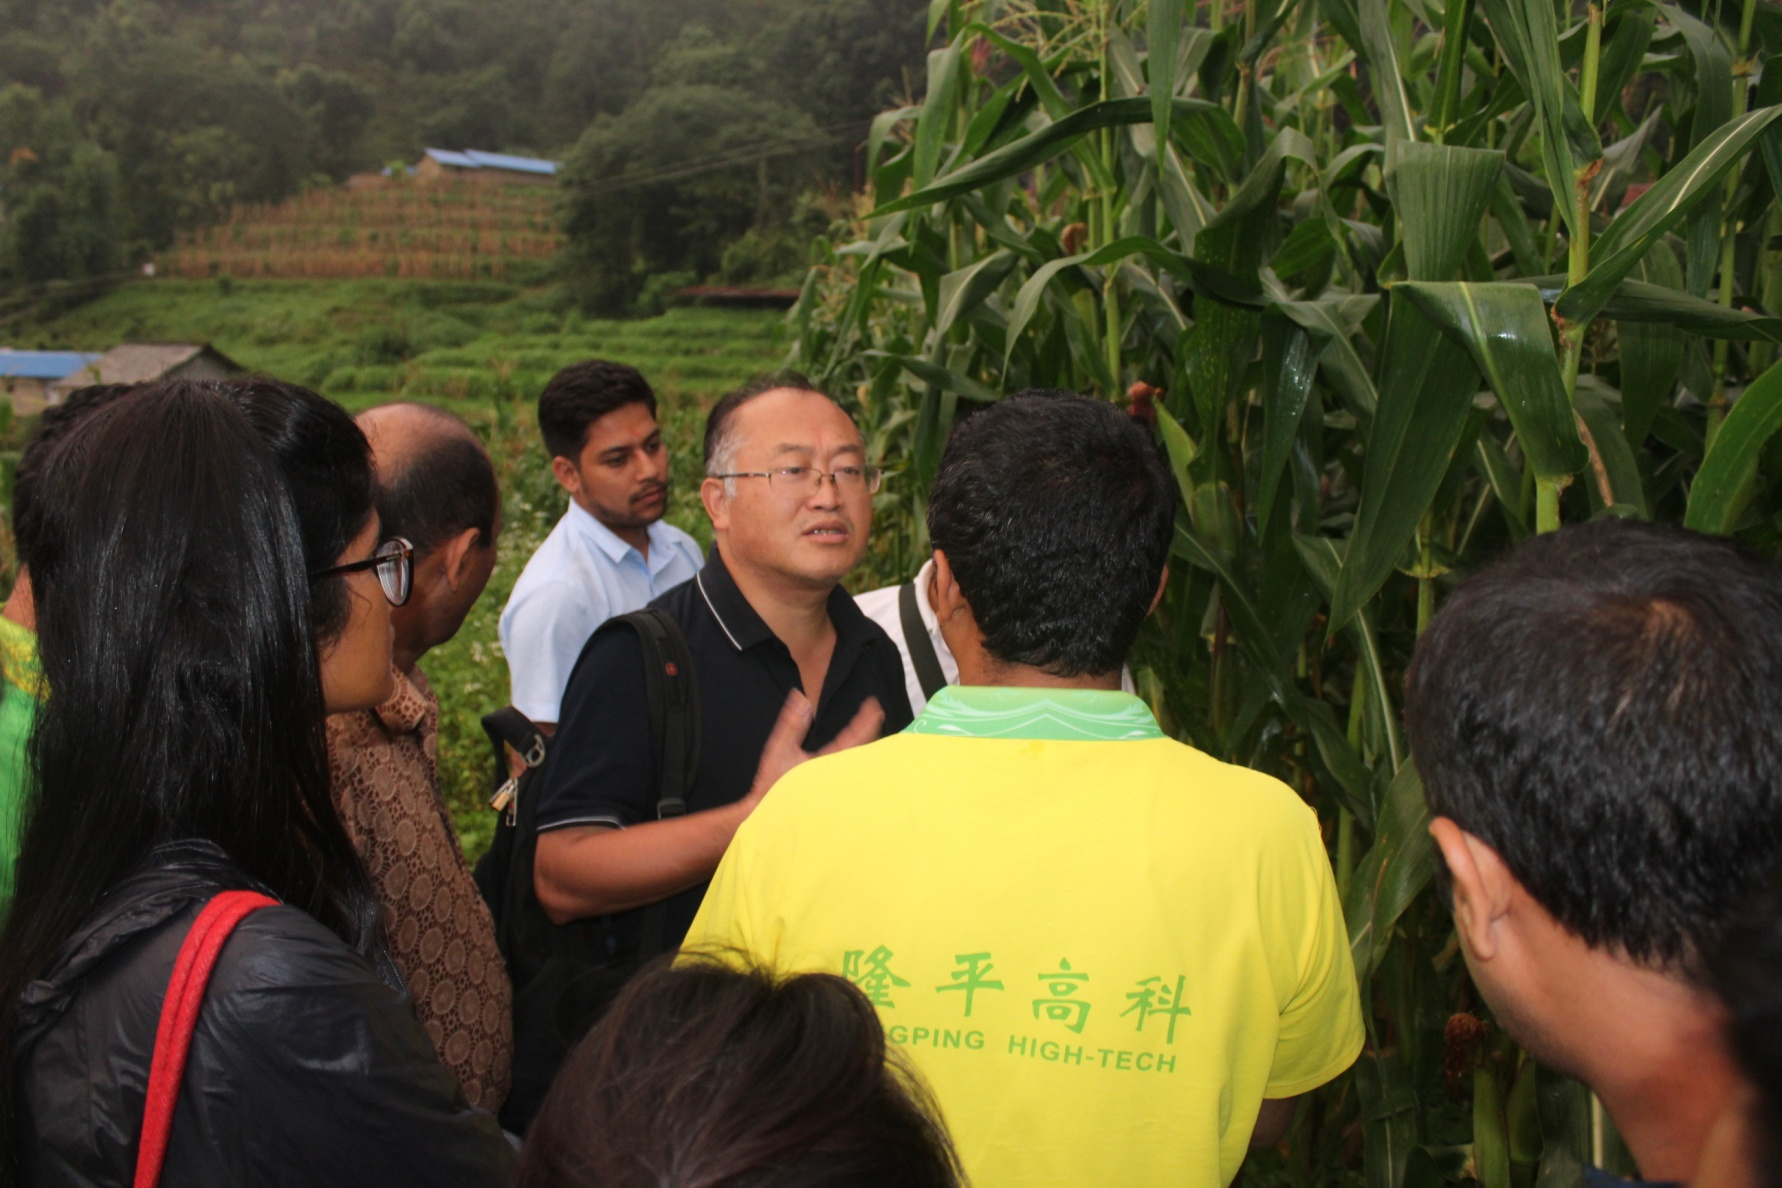
\includegraphics[width=.25\linewidth]{./images/maize_experiment_field_lumle} }\newline\subfloat[Maize experiment field with yield testing\label{fig:team-field-trips3}]{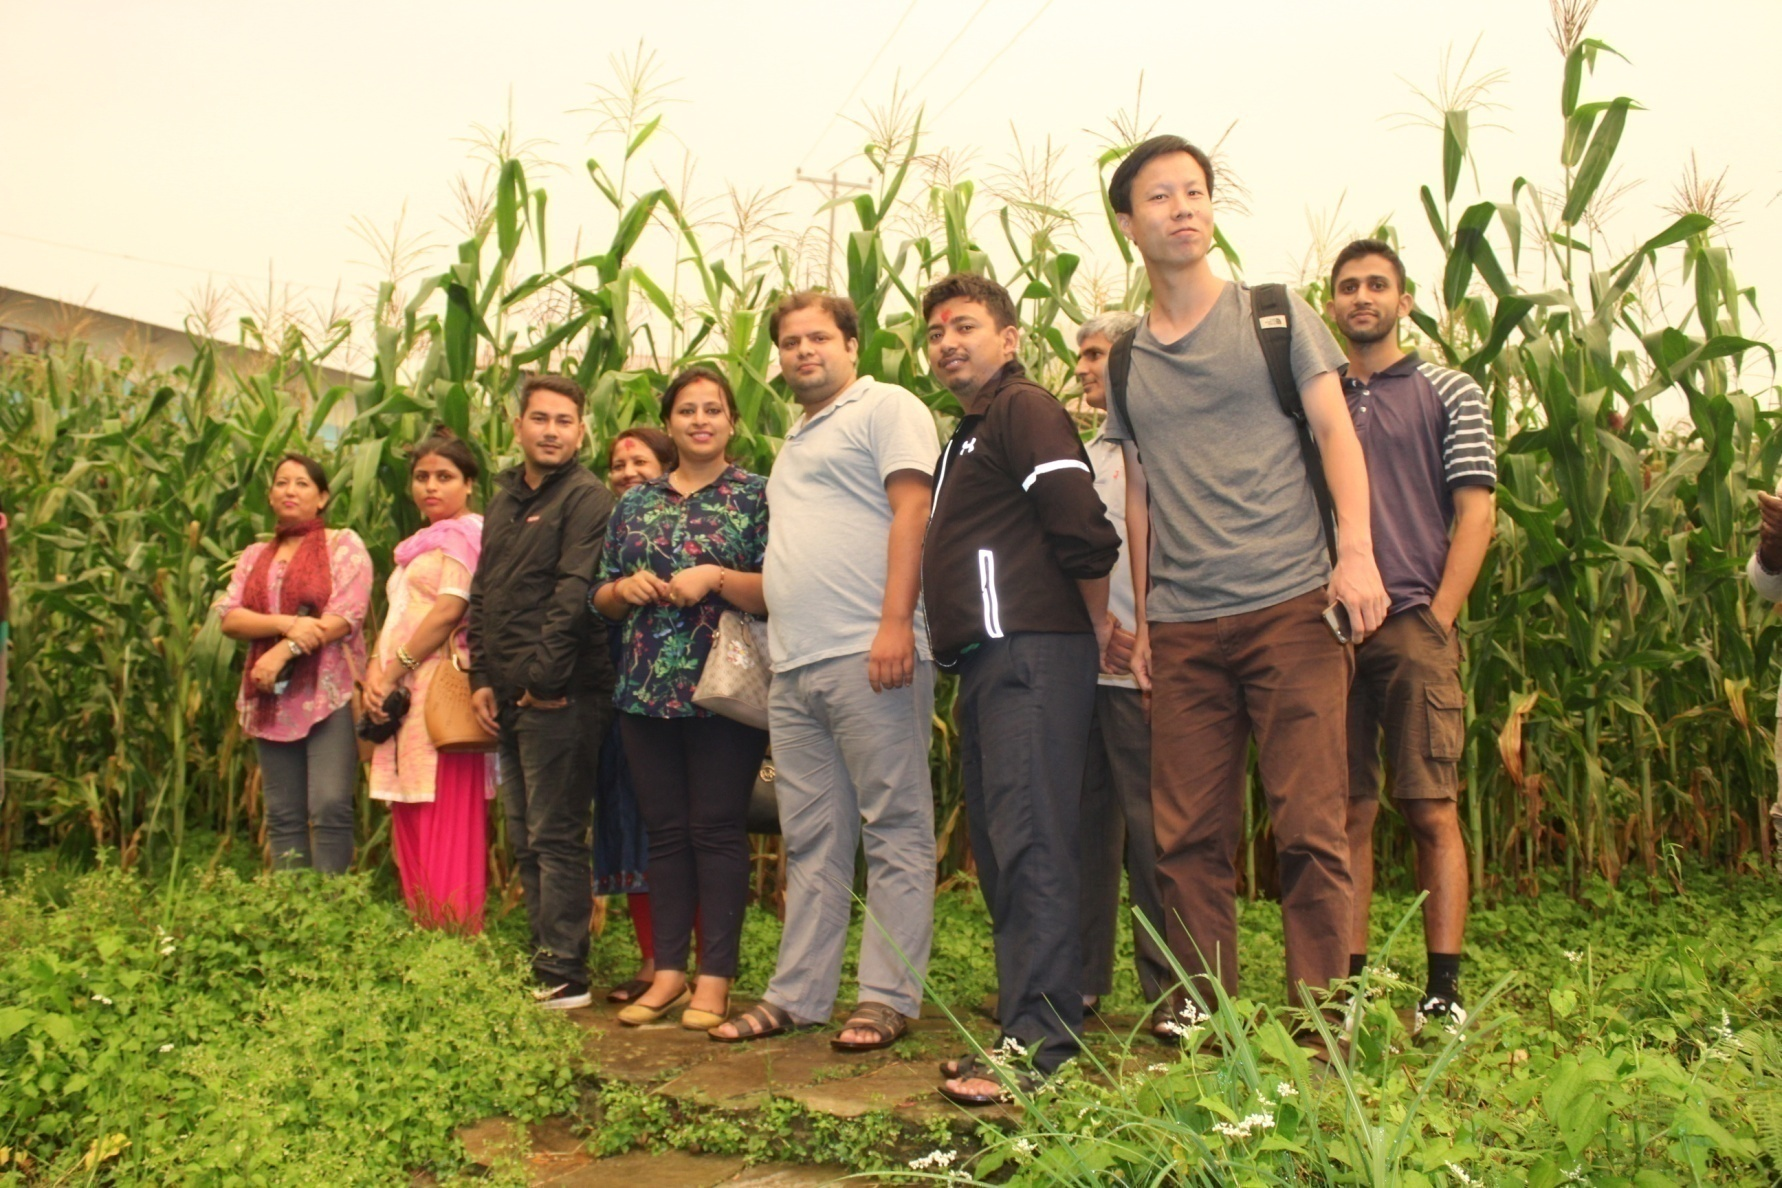
\includegraphics[width=.25\linewidth]{./images/maize_experiment_field_lumle2} }\caption{Gallery of images showing team during excursion visit to RARS, Lumle}\label{fig:team-field-trips}
\end{figure}

\end{frame}

\hypertarget{bibliography}{%
\section{Bibliography}\label{bibliography}}

\begin{frame}{References}
\protect\hypertarget{references}{}

\end{frame}

\begin{frame}[standout]{}
\protect\hypertarget{section-6}{}

Thanks for sliding!

\end{frame}




\end{document}
